\chapter{Clustering}

In the exercises in this chapter you will first use a visualization of the k-means clustering that helps to understand how it works. You will then apply the k-means clustering as a machine learning method to segment plants based on their color and than on features of the scratch-assay-images.

\section{K-means clustering}

Open the file {\tt Visualizing K-Means Clustering.html} from the folder {\tt 01-k-means-visualization}. The applet allows you to see the k-means clustering at work. You can select different strategies for the initial mean-values and different data--sets. You can follow the k-means algorithm step by step. 

Run the k-means algorithm with different initialization strategies and on different data--sets and answer the following questions.

\begin{enumerate}
\item What influence do you think the selection of the initial mean values has on the clustering result ?
\begin{verbatim}







\end{verbatim}
\item Does the k-means algorithm always converge, i.e. does it always come to a point where further iterations do not change the result anymore?
\begin{verbatim}


\end{verbatim}
\item Is the result of the clustering always the same, no matter what the choice of the initial means is?
\begin{verbatim}


\end{verbatim}
\item Does the k-means clustering work as expected on the {\tt Smiley Face} data--set? What is the reason it does or does not work as expected?
\begin{verbatim}









\end{verbatim}
\end{enumerate}

\section{Using K-means clustering for color segmentation}

Images of Arabidopsis thaliana are taken in regular intervals. The aim is to measure the speed with which the area of the rosette of leaves augments under different conditions and treatments. You will use k-means clustering to segment the rosettes of the plants. You will create a color-stack using an appropriate color-space (RGB, HSB or Lab) and use the {\tt k-means segmentation} tool. 

\begin{figure}[!htb]
 \centering
 \includegraphics[width=8cm]{arabidopsis}
 \caption{Arabidopsis plant at 3 different stages.}
 \label{figure:arabidopsis}
\end{figure}

\begin{enumerate}
\item Run {\tt FIJI} and open one of the images from the folder {\tt 03 - plants}. Convert the image to a color stack using one of the commands {\tt RGB Stack}, {\tt HSB Stack} or {\tt Lab Stack} from the menu {\tt Image>Type}.  Run the {\tt k-means segmentation} tool from the menu {\tt Plugins>k-means experiment>k-means segmentation}.
\begin{figure}[!htb]
 \centering
 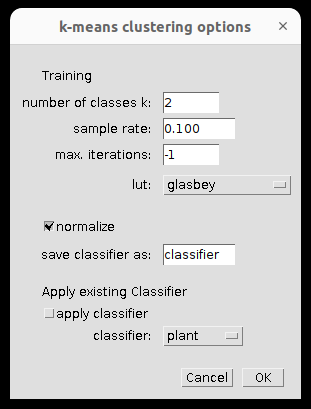
\includegraphics[width=4cm]{color_clustering}
 \caption{The options of the k-means segmentation command.}
 \label{figure:color_clustering}
\end{figure}
\item How many clusters do you think are appropriate? 
\begin{verbatim}
Number of clusters:

\end{verbatim}
Configure the k-means segmentation to use the number of clusters you have decided to use and run it on the stack. The value of a pixel in the result image corresponds to the cluster to which the pixel belongs. 

What is the class of the color values belonging to the plant?
\begin{verbatim}
Class of plant:

\end{verbatim}
What is the class of the color values belonging to the small red reference object in the form of a ball?
\begin{verbatim}
Class of reference object:

\end{verbatim}

\item Create a selection (roi) from the result of the pixel classification and display it on the original input image. Use the commands {\tt select label(s)} and {\tt Keep largest region} to isolate the target label. Then open the threshold adjuster (shift-t) and run the command {\tt create selection}. Transfer the selection to the original input image (restore selection or use the roi-manager). How good is the selection? Measure the area of the surface of the plant.
\begin{verbatim}
Area of the plant:

\end{verbatim}
\item Check the log--window. The clustering algorithm has written the k mean-vectors into the log. What are their values?
\begin{verbatim}
k mean vectors:




\end{verbatim}

\item Apply the saved k-means classifier on a different image from the plant-series.
\end{enumerate}

\section{Using K-means clustering on other features}

We can use the k-means clustering not only with colors but also with other features. 

\begin{enumerate}
\item Open an image from {\tt scratch-assay}-folder. Create two or three feature images from the input image for example by using FeatureJ. Use appropriate scales when creating the features. Use {\tt Image>Color>Merge Channels...} to create a stack of the feature images. Run the k-means clustering on the stack. What is the area of the gap?
\begin{verbatim}
Area of the gap:

\end{verbatim}

\end{enumerate}

